% ==================================================================
%  徐森林、薛春华《数学分析》（第一册）
%  \S3.5  应用导数研究函数之一: 单调性、极值、最值
% ==================================================================
%  源：原书印刷页 206-221（PDF 物理页 212-227）
%  底本：PaddleOCR-VL-1.6 + 高清影印比对校订
%  规范：全西文半角标点；单一落盘出口 _texout.py
% ==================================================================
\section{应用导数研究函数之一: 单调性、极值、最值}\label{sec:3.5}

作为 Fermat 定理、Rolle 定理、Lagrange 中值定理与 Cauchy 中值定理的应用, 我们来研究函数的单调性、极值、最值以及凹凸性.

\begin{theorem}\label{thm:3.5.1}
设 $I$ 为区间, $f$ 在 $I$ 上连续, 在 $\mathring{I}$ 内可导, 且 $f'(x)>0(<0)$, 则 $f$ 在 $I$ 上严格增(减). 反之不真.
\end{theorem}

\begin{proof}
$\forall x_{1},x_{2}\in I$, $x_{1}<x_{2}$, 由 Lagrange 中值定理, $\exists\xi\in(x_{1},x_{2})\subset I$, s.t.
\[
\frac{f(x_{2})-f(x_{1})}{x_{2}-x_{1}}=f'(\xi)>0,
\]
所以, $f(x_{1})<f(x_{2})$, 即 $f$ 在 $I$ 上严格增.

当 $f'(x)<0$ 时, 类似证明, 或用 $-f$ 代替 $f$ 即可证得.

反之不真, 有反例: $f(x)=x^{3}$ 在 $(-\infty,+\infty)$ 上严格增, 但 $f'(0)=3x^{2}|_{x=0}=0$.
\end{proof}

\begin{theorem}\label{thm:3.5.2}
设 $I$ 为区间, $f$ 在 $I$ 上连续, 在 $\mathring{I}$ 内可导, 则
\[
f\ \text{在}\ I\ \text{上单调增(减)}\Longleftrightarrow f'(x)\geqslant 0(\leqslant 0),\ \forall x\in\mathring{I}.
\]
\end{theorem}

\begin{proof}
($\rightarrow$) $\forall x\in\mathring{I}$, 因 $f$ 在 $I$ 上单调增, 故
\[
\frac{f(x+\Delta x)-f(x)}{\Delta x}\geqslant 0,
\]
所以,
\[
f'(x)=\lim_{\Delta x\to 0}\frac{f(x+\Delta x)-f(x)}{\Delta x}\geqslant 0.
\]

($\leftarrow$) $\forall x_{1},x_{2}\in I$, $x_{1}<x_{2}$, 由 Lagrange 中值定理知, $\exists\xi\in(x_{1},x_{2})\subset\mathring{I}$, s.t.
\[
\frac{f(x_{2})-f(x_{1})}{x_{2}-x_{1}}=f'(\xi)\geqslant 0,
\]
所以, $f(x_{1})\leqslant f(x_{2})$, 即 $f$ 在 $I$ 上单调增.

当 $f'(x)\leqslant 0$ 时, 类似证明, 或用 $-f$ 代替 $f$ 即可证得.
\end{proof}

\begin{theorem}\label{thm:3.5.3}
设 $I$ 为区间, $f$ 在 $I$ 上连续, 在 $\mathring{I}$ 内可导, 则 $f$ 在 $I$ 上严格增(减) $\Longleftrightarrow$
(1) $f'(x)\geqslant 0(\leqslant 0)$, $\forall x\in\mathring{I}$; (2) $\{x\in\mathring{I}\mid f'(x)=0\}$ 不构成区间, 或在任何非退化区间 $I_{1}\subset\mathring{I}$ 上, $f'(x)\neq 0$.
\end{theorem}

\begin{proof}
($\rightarrow$) (1) 因为 $f$ 严格增, 当然是单调增, 由定理~\ref{thm:3.5.2} 知, $f'(x)\geqslant 0$, $\forall x\in\mathring{I}$.

(2) (反证) 假设有非退化区间 $I_{1}\subset\mathring{I}$, s.t. $f'(x)=0$, $\forall x\in I_{1}$, 则由推论~\ref{cor:3.3.1} 知, $f(x)=$ 常数, $\forall x\in I_{1}$, 这与 $f$ 严格增相矛盾.

($\leftarrow$) 由右边的条件(1)与定理~\ref{thm:3.5.2} 推得 $f$ 单调增, 故 $\forall x_{1},x_{2}\in I$, $x_{1}<x_{2}$, 有 $f(x_{1})\leqslant f(x_{2})$.

如果 $f(x_{1})=f(x_{2})$, 由 $f$ 单调增知, $f(x)=f(x_{1})$, $\forall x\in[x_{1},x_{2}]$, 所以 $f'(x)=0$, $\forall x\in(x_{1},x_{2})=I_{1}$, 这与右边条件(2)相矛盾. 因此, $\forall x_{1},x_{2}\in I$, $x_{1}<x_{2}$, 有
\[
f(x_{1})<f(x_{2}),
\]
这就证明了 $f$ 在 $I$ 上是严格增的.

关于严格减的情形可类似证明, 或用 $-f$ 代替 $f$ 即可证得.
\end{proof}

\begin{example}\label{ex:3.5.1}
证明 $f(x)=x^{3}$ 在 $(-\infty,+\infty)$ 上是严格增的.
\end{example}

\begin{proof}[证法 1]
因为 $f'(x)=3x^{2}\geqslant 0$, 且 $\{x\mid f'(x)=3x^{2}=0\}=\{0\}$ 不构成区间, 根据定理~\ref{thm:3.5.3} 知, $f(x)=x^{3}$ 在 $(-\infty,+\infty)$ 是严格增的.
\end{proof}

\begin{proof}[证法 2]
对 $x_{1}<x_{2}$, 有
\[
\begin{aligned}
x_{2}^{3}-x_{1}^{3}&=(x_{2}-x_{1})(x_{2}^{2}+x_{2}x_{1}+x_{1}^{2})\\
&=(x_{2}-x_{1})[(|x_{2}|-|x_{1}|)^{2}+2|x_{2}x_{1}|+x_{2}x_{1}]>0,
\end{aligned}
\]
故 $f(x_{1})=x_{1}^{3}<x_{2}^{3}=f(x_{2})$, 即 $f$ 在 $(-\infty,+\infty)$ 是严格增的.
\end{proof}

\begin{example}\label{ex:3.5.2}
证明 $f(x)=x-\sin x$ 在 $(-\infty,+\infty)$ 上严格增.
\end{example}

\begin{proof}
由于 $f'(x)=1-\cos x\geqslant 0$, 且 $\{x\mid f'(x)=1-\cos x=0\}=\{2k\pi\mid k=0,\pm 1,\pm 2,\cdots\}$ 不构成区间, 根据定理~\ref{thm:3.5.3} 知, $f(x)=x-\sin x$ 在 $(-\infty,+\infty)$ 是严格增的.
\end{proof}

\begin{example}\label{ex:3.5.3}
讨论函数 $f(x)=x^{3}-x=x(x+1)(x-1)$ 的单调区间.
\end{example}

\begin{solution}
由于 $f'(x)=3x^{2}-1=(\sqrt{3}x+1)(\sqrt{3}x-1)$, 故驻点为 $x_{1}=-\frac{1}{\sqrt{3}}$, $x_{2}=\frac{1}{\sqrt{3}}$. 应用定理~\ref{thm:3.5.3} 以及下表知, $f$ 在 $\left(-\infty,-\frac{1}{\sqrt{3}}\right)$ 中严格增; 在 $\left(-\frac{1}{\sqrt{3}},\frac{1}{\sqrt{3}}\right)$ 中严格减; 在 $\left(\frac{1}{\sqrt{3}},+\infty\right)$ 中又严格增.

列成表如下:
\begin{center}
\begin{tabular}{|c|c|c|c|c|c|c|c|}
\hline
$x$ & $-\infty$ & & $-\frac{1}{\sqrt{3}}$ & & $\frac{1}{\sqrt{3}}$ & & $+\infty$ \\
\hline
$\sqrt{3}x+1$ & & $-$ & & $+$ & & $+$ & \\
\hline
$\sqrt{3}x-1$ & & $-$ & & $-$ & & $+$ & \\
\hline
$f'(x)$ & & $+$ & & $-$ & & $+$ & \\
\hline
$f(x)$ & & $\nearrow$ & & $\searrow$ & & $\nearrow$ & \\
\hline
\end{tabular}
\end{center}

\begin{figure}[htbp]
\centering
\begin{minipage}[t]{0.50\textwidth}
\begin{gather*}
f(-1)=f(0)=f(1)=0,\\
f\Big(\frac{1}{\sqrt{3}}\Big)=-\frac{2}{3\sqrt{3}}=-\frac{2\sqrt{3}}{9},\\
f\Big(-\frac{1}{\sqrt{3}}\Big)=-f\Big(\frac{1}{\sqrt{3}}\Big)=\frac{2\sqrt{3}}{9},\\
\lim_{x\to-\infty}f(x)=\lim_{x\to-\infty}x^{3}\Big(1-\frac{1}{x^{2}}\Big)=-\infty,\\
\lim_{x\to+\infty}f(x)=\lim_{x\to+\infty}x^{3}\Big(1-\frac{1}{x^{2}}\Big)=+\infty.
\end{gather*}
\end{minipage}
\hfill
\begin{minipage}[t]{0.47\textwidth}
\centering
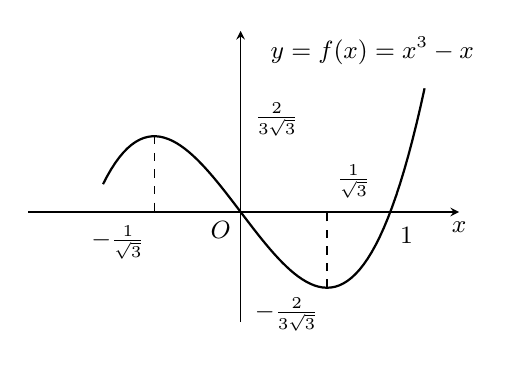
\begin{tikzpicture}[>=stealth,font=\small,x=1.9cm,y=2.5cm,
  baseline=(current bounding box.north)]
  \draw[->] (-1.42,0) -- (1.46,0) node[below] {$x$};
  \draw[->] (0,-0.56) -- (0,0.92);
  \node[below left] at (0,0) {$O$};
  \draw[thick] plot[domain=-0.92:1.23,samples=80] (\x,{(\x)^3-(\x)});
  \draw[dashed] (-0.577,0.385) -- (-0.577,0);
  \draw[dashed] (0.577,-0.385) -- (0.577,0);
  \node[right] at (0.03,0.47) {$\frac{2}{3\sqrt{3}}$};
  \node[right] at (0.03,-0.52) {$-\frac{2}{3\sqrt{3}}$};
  \node[below left] at (-0.577,-0.02) {$-\frac{1}{\sqrt{3}}$};
  \node[above right] at (0.577,0.02) {$\frac{1}{\sqrt{3}}$};
  \node[below right] at (1.0,-0.03) {$1$};
  \node[above] at (0.88,0.70) {$y=f(x)=x^{3}-x$};
\end{tikzpicture}
\caption{}\label{fig:3.5.1}
\end{minipage}
\end{figure}

由上可见, $-\frac{1}{\sqrt{3}}$ 与 $\frac{1}{\sqrt{3}}$ 分别为 $f(x)$ 在 $(-\infty,+\infty)$ 上的极大值点与极小值点 (如图~\ref{fig:3.5.1} 所示).
\end{solution}

\begin{example}\label{ex:3.5.4}
设 $n\in\mathbb{N}$, 证明:
\[
\mathrm{e}^{x}>1+\frac{x}{1!}+\frac{x^{2}}{2!}+\cdots+\frac{x^{n}}{n!},\quad\forall x>0.
\]
\end{example}

\begin{proof}
(数学归纳法) 当 $n=1$ 时, 令 $\varphi(x)=\mathrm{e}^{x}-(1+x)$, $x\geqslant 0$, 则 $\varphi'(x)=\mathrm{e}^{x}-1>0$, $x>0$. 这表明 $\varphi$ 在 $[0,+\infty)$ 上是严格增的. 于是,
\[
\mathrm{e}^{x}-(1+x)=\varphi(x)>\varphi(0)=0,
\]
\[
\mathrm{e}^{x}>1+x,\ x>0.
\]
不等式成立.

假设 $n=k$ 时, 有
\[
\mathrm{e}^{x}>1+\frac{x}{1!}+\frac{x^{2}}{2!}+\cdots+\frac{x^{k}}{k!},\quad x>0,
\]
则当 $n=k+1$ 时, 令
\[
\psi(x)=\mathrm{e}^{x}-\Big[1+\frac{x}{1!}+\frac{x^{2}}{2!}+\cdots+\frac{x^{k+1}}{(k+1)!}\Big],\quad x\geqslant 0.
\]
依归纳假设,
\[
\psi'(x)=\mathrm{e}^{x}-\Big(1+\frac{x}{1!}+\cdots+\frac{x^{k}}{k!}\Big)>0,\quad x>0.
\]
这表明 $\psi$ 在 $[0,+\infty)$ 上是严格增的. 于是,
\[
\psi(x)>\psi(0)=0,
\]
即
\[
\mathrm{e}^{x}>1+\frac{x}{1!}+\frac{x^{2}}{2!}+\cdots+\frac{x^{k}}{k!},\quad x>0.
\]
\end{proof}

\begin{example}\label{ex:3.5.5}
证明: $\frac{2}{\pi}\leqslant\frac{\sin x}{x}<1$, $x\in\left(0,\frac{\pi}{2}\right]$.
\end{example}

\begin{proof}
令 $f(x)=\frac{\sin x}{x}$, 则 $f'(x)=\frac{x\cos x-\sin x}{x^{2}}=\cos x\cdot\frac{x-\tan x}{x}<0$, $x\in\left(0,\frac{\pi}{2}\right)$, 从而 $f(x)$ 在 $\left(0,\frac{\pi}{2}\right]$ 上严格减. 又因为 $\lim\limits_{x\to 0}\frac{\sin x}{x}=1$, 所以
\[
\frac{2}{\pi}=\frac{\sin\frac{\pi}{2}}{\frac{\pi}{2}}\leqslant\frac{\sin x}{x}<1,\quad x\in\left(0,\frac{\pi}{2}\right].
\]
\end{proof}

\begin{example}\label{ex:3.5.6}
设 $f$ 在 $(a,+\infty)$ 上有有界的导函数. 证明: 存在常数 $C$ 与 $x_{0}$, 当 $x\geqslant x_{0}$ 时, $f(x)<Cx$.
\end{example}

\begin{proof}
设 $|f'(x)|\leqslant M$, $\forall x\in(a,+\infty)$. 取定 $x_{0}>0$, 再取 $C>\max\left\{M,\frac{f(x_{0})}{x_{0}}\right\}$. 令 $F(x)=f(x)-Cx$, 则
\[
F'(x)=f'(x)-C<0,
\]
根据定理~\ref{thm:3.5.1} 知, $F(x)$ 在 $(a,+\infty)$ 上严格减. 所以,
\[
f(x)-Cx=F(x)\leqslant F(x_{0})=f(x_{0})-Cx_{0}<0,\ \forall x\geqslant x_{0},
\]
即
\[
f(x)<Cx,\ \forall x\geqslant x_{0}.
\]
\end{proof}

\begin{example}\label{ex:3.5.7}
设 $f$ 在 $[a,+\infty)$ 上连续, 在 $(a,+\infty)$ 内可导, $f(a)<0$, 且当 $x>a$ 时, $f'(x)>k>0$. 证明: $f$ 有惟一的零点.
\end{example}

\begin{proof}
由 $f(a)<0$ 与 $k>0$ 知, $a-\frac{f(a)}{k}>a$. 在 $\left[a,a-\frac{f(a)}{k}\right]$ 上应用 Lagrange 中值定理, $\exists\xi\in\left(a,a-\frac{f(a)}{k}\right)$, s.t.
\[
\begin{aligned}
f\Big(a-\frac{f(a)}{k}\Big)-f(a)&=f'(\xi)\Big[\Big(a-\frac{f(a)}{k}\Big)-a\Big]\\
&=f'(\xi)\cdot\frac{-f(a)}{k}>k\cdot\frac{-f(a)}{k}\\
&=-f(a).
\end{aligned}
\]
因此得到 $f\left(a-\frac{f(a)}{k}\right)>0$. 根据零值定理可知, $\exists c\in\left(a,a-\frac{f(a)}{k}\right)$, s.t. $f(c)=0$.

另一方面, 由题设知, 当 $x>a$ 时, $f'(x)>k>0$, 因此, $f$ 在 $[a,+\infty)$ 上严格增, 从而 $f(x)=0$ 至多只有一个零点.

综上所述可推得 $f$ 有惟一的零点.
\end{proof}

\begin{example}\label{ex:3.5.8}
当 $x>0$ 时, 证明:
\[
\begin{aligned}
x-\frac{x^{3}}{3!}+\frac{x^{5}}{5!}-\cdots-\frac{x^{4k+3}}{(4k+3)!}&<\sin x\\
<x-\frac{x^{3}}{3!}+\frac{x^{5}}{5!}-\cdots-\frac{x^{4k-1}}{(4k-1)!}&+\frac{x^{4k+1}}{(4k+1)!},\\
1-\frac{x^{2}}{2!}+\frac{x^{4}}{4!}-\cdots-\frac{x^{4k+2}}{(4k+2)!}&<\cos x\\
<1-\frac{x^{2}}{2!}+\frac{x^{4}}{4!}-\cdots-\frac{x^{4k+2}}{(4k+2)!}&+\frac{x^{4k+4}}{(4k+4)!}.
\end{aligned}
\]
\end{example}

\begin{proof}
(1) 令 $F_{0}(x)=x-\sin x$, 则 $F'_{0}(x)=1-\cos x\geqslant 0$, 又 $\{x\in(0,+\infty)\mid F'(x)=1-\cos x=0\}=\{2k\pi\mid k\in\mathbb{N}\}$ 不构成区间, 根据定理~\ref{thm:3.5.3} 知, $F_{0}$ 在 $[0,+\infty)$ 上严格增. 于是,
\[
x-\sin x=F_{0}(x)>F(0)=0,
\]
即
\[
\sin x<x,\quad\forall x>0.
\]

(2) 令 $G_{0}(x)=\cos x-1+\frac{x^{2}}{2}$, 则由(1)知,
\[
G'_{0}(x)=-\sin x+x=x-\sin x>0,\quad\forall x>0,
\]
所以, $G_{0}(x)$ 在 $[0,+\infty)$ 上严格增. 于是,
\[
\cos x-1+\frac{x^{2}}{2}=G(x)>G(0)=0,
\]
即
\[
\cos x>1-\frac{x^{2}}{2},\quad\forall x>0.
\]

(3) 令 $H_{0}(x)=\sin x-x+\frac{x^{3}}{3!}$, 则由(2)知,
\[
H'_{0}(x)=\cos x-1+\frac{x^{2}}{2}>0,\quad\forall x>0,
\]
所以, $H_{0}(x)$ 在 $[0,+\infty)$ 上严格增. 于是,
\[
\sin x-x+\frac{x^{3}}{3!}=H(x)>H(0)=0,
\]
即
\[
\sin x>x-\frac{x^{3}}{3!},\quad\forall x>0.
\]

(4) 令 $Q_{0}(x)=1-\frac{x^{2}}{2!}+\frac{x^{4}}{4!}-\cos x$, 则由(3)知,
\[
Q'_{0}(x)=\sin x-x+\frac{x^{3}}{3!}>0,\quad\forall x>0,
\]
所以, $Q_{0}(x)$ 在 $[0,+\infty)$ 上严格增. 于是,
\[
1-\frac{x^{2}}{2!}+\frac{x^{4}}{4!}-\cos x=Q(x)>Q(0)=0,
\]
即
\[
\cos x<1-\frac{x^{2}}{2!}+\frac{x^{4}}{4!},\quad\forall x>0.
\]

余下请读者仿照以上(1)～(4)依次构造函数 $F_{l}(x)$, $G_{l}(x)$, $H_{l}(x)$, $Q_{l}(x)$, $l=1,2,\cdots$, 并应用归纳法完成不等式的全部证明.
\end{proof}

\begin{remark}\label{rem:3.5.1}
例~\ref{ex:3.5.4}、例~\ref{ex:3.5.5}、例~\ref{ex:3.5.8} 中各函数不等式的证法有一个共同之点, 就是先将不等式两边的函数移到一边去, 并构造一个新函数, 再应用导数证明新函数的单调性, 然后, 证明新函数大于零或小于零. 最终将移过来的函数移回去便得要证的不等式.
\end{remark}

Fermat 定理指出: 如果函数 $f$ 在 $x_{0}$ 达极值且可导, 则 $x_{0}$ 必为 $f$ 的驻点. 因此, $x_{0}$ 为 $f$ 的驻点是 $f$ 在 $x_{0}$ 可导下达到极值的必要条件, 但它不是充分条件. $y=f(x)=x^{3}$, $x_{0}=0$ 就是一个反例. 下面我们将给出两个达到极值的充分条件.

\begin{theorem}[极值的充分条件之一]\label{thm:3.5.4}
设 $f$ 在 $I$ 上有定义, $x_{0}\in\mathring{I}$ 为 $f$ 的连续点.

(1) 如果
\[
f'(x)\left\{
\begin{aligned}
&>0,\ x\in(x_{0}-\delta,x_{0}),\\
&<0,\ x\in(x_{0},x_{0}+\delta),
\end{aligned}
\right.
\]
则 $x_{0}$ 为 $f$ 的一个严格极大值点;

(2) $\exists\delta>0$, s.t.
\[
f'(x)\left\{
\begin{aligned}
&<0,\ x\in(x_{0}-\delta,x_{0}),\\
&>0,\ x\in(x_{0},x_{0}+\delta),
\end{aligned}
\right.
\]
则 $x_{0}$ 为 $f$ 的一个严格极小值点.
\end{theorem}

\begin{proof}
(1) 由定理~\ref{thm:3.5.1} 知, $f$ 在 $(x_{0}-\delta,x_{0}]$ 严格增, 所以 $f(x)<f(x_{0})$, $\forall x\in(x_{0}-\delta,x_{0})$; 再由定理~\ref{thm:3.5.1} 知, $f$ 在 $[x_{0},x_{0}+\delta)$ 上严格减, 所以 $f(x)<f(x_{0})$, $\forall x\in(x_{0},x_{0}+\delta)$. 这就证明了 $x_{0}$ 为 $f$ 的严格极大值点.

(2) 类似(1)证明, 或用 $-f$ 代替 $f$ 即可证得.
\end{proof}

读者自然会问: 如果 $x_{0}$ 为 $f$ 的驻点, 应再附加什么条件, $x_{0}$ 为 $f$ 的极值点, 是极大值点还是极小值点?

\begin{theorem}[极值的充分条件二]\label{thm:3.5.5}
设 $f$ 在 $I$ 上有定义, $x_{0}\in\mathring{I}$ 为 $f$ 的一个驻点, 即 $f'(x_{0})=0$. 进一步, 设 $f''(x_{0})$ 存在有限, 则:

(1) 当 $f''(x_{0})<0$ 时, $x_{0}$ 为 $f$ 的一个严格极大值点;

(2) 当 $f''(x_{0})>0$ 时, $x_{0}$ 为 $f$ 的一个严格极小值点.
\end{theorem}

\begin{proof}
(1) 因为
\[
\lim_{x\to x_{0}}\frac{f'(x)}{x-x_{0}}=\lim_{x\to x_{0}}\frac{f'(x)-f'(x_{0})}{x-x_{0}}=f''(x_{0})<0,
\]
所以, $\exists\delta>0$, s.t. 当 $0<|x-x_{0}|<\delta$ 时,
\[
\frac{f'(x)}{x-x_{0}}<0.
\]
由此可知,
\[
f'(x)\left\{
\begin{aligned}
&>0,\ x\in(x_{0}-\delta,x_{0}),\quad f\ \text{严格增},\\
&<0,\ x\in(x_{0},x_{0}+\delta),\quad f\ \text{严格减}.
\end{aligned}
\right.
\]
再由 $f$ 在 $x_{0}$ 可导, 从定理~\ref{thm:3.1.2} 知, $f$ 在 $x_{0}$ 连续. 根据定理~\ref{thm:3.5.4}(1) 推得, $x_{0}$ 为 $f$ 的极大值点.

(2) 类似(1)证明, 或用 $-f$ 代替 $f$ 即可证得.
\end{proof}

\begin{example}\label{ex:3.5.9}
上面两个定理只是判断严格极值的充分条件. 有这样的函数 $f$, 在它的严格极小值点 $x=0$ 的任何一侧都不具有单调的性质. 考察函数
\[
f(x)=\left\{
\begin{aligned}
&x\sin\frac{1}{x}+2|x|,\quad x\neq 0,\\
&0,\quad x=0.
\end{aligned}
\right.
\]
它是一个处处连续的偶函数. 因为 $\left|x\sin\frac{1}{x}\right|\leqslant|x|<2|x|$, $x\neq 0$, 所以 $f(x)>0=f(0)$.

从而 0 为 $f$ 的严格极小值(也是严格最小值). 但是, 当 $x>0$ 时,
\[
f'(x)=\sin\frac{1}{x}-\frac{1}{x}\cos\frac{1}{x}+2,
\]
所以, 对 $\forall n\in\mathbb{N}$, 有
\[
f'\left(\frac{1}{n\pi}\right)=0-n\pi\cdot(-1)^{n}+2=2+(-1)^{n+1}n\pi.
\]
当 $n$ 从 $1,2,3,\cdots$ 依次地跑过时, $f'\left(\frac{1}{n\pi}\right)$ 正负交替地改变符号, 因此 $\forall\delta>0$, 函数 $f$ 在区间 $(0,\delta)$ 上都不是单调的; 在 $(-\delta,0)$ 上也是这样.
\end{example}

\begin{corollary}\label{cor:3.5.1}
设 $f$ 在 $x_{0}$ 处 2 阶可导, $x_{0}$ 为 $f$ 的极大(小)值点, 则 $f''(x_{0})\leqslant 0(\geqslant 0)$.
\end{corollary}

\begin{proof}
(反证) 假设 $f''(x_{0})>0$, 由定理~\ref{thm:3.5.5}(2) 知, $x_{0}$ 为 $f$ 的严格极小值点, 又因为 $x_{0}$ 为 $f$ 的极大值点, 故 $\exists\delta>0$, 当 $0<|x-x_{0}|<\delta$ 时, 有
\[
f(x_{0})<f(x)\leqslant f(x_{0}),
\]
矛盾.

关于 $f''(x_{0})\geqslant 0$ 的情形可类似证明, 或用 $-f$ 代替 $f$ 即可证得.
\end{proof}

现在来讨论函数的最大值与最小值的问题, 这个问题有重大的理论价值与应用价值.

已经知道, 有界闭区间 $[a,b]$ 上的连续函数 $f$ 必达到它的最大值与最小值. 关于 $f$ 的最值有下面的定理.

\begin{theorem}\label{thm:3.5.6}
设 $f$ 为 $[a,b]$ 上的连续函数, 在 $(a,b)$ 内部, 除 $s_{1},s_{2},\cdots,s_{k}$ 外都可导, $t_{1},t_{2},\cdots,t_{l}$ 为 $f$ 的全部驻点, 则
\[
\begin{aligned}
\max_{a\leqslant x\leqslant b}f(x)&=\max\{f(a),f(s_{1}),\cdots,f(s_{k}),f(t_{1}),\cdots,f(t_{l}),f(b)\},\\
\min_{a\leqslant x\leqslant b}f(x)&=\min\{f(a),f(s_{1}),\cdots,f(s_{k}),f(t_{1}),\cdots,f(t_{l}),f(b)\}.
\end{aligned}
\]
\end{theorem}

\begin{proof}
因为 $f$ 为 $[a,b]$ 上的连续函数, 根据最值定理~\ref{thm:2.5.3} 知, $f$ 必达到它的最大值与最小值. 这最值点或者为 $a,b$; 或者为 $(a,b)$ 内部的不可导点; 或者为 $(a,b)$ 内部的极值点. 根据 Fermat 定理, 这种极值点必为 $f$ 的驻点. 综合上述得到
\[
\begin{aligned}
\max_{a\leqslant x\leqslant b}f(x)&=\max\{f(a),f(s_{1}),\cdots,f(s_{k}),f(t_{1}),\cdots,f(t_{l}),f(b)\},\\
\min_{a\leqslant x\leqslant b}f(x)&=\min\{f(a),f(s_{1}),\cdots,f(s_{k}),f(t_{1}),\cdots,f(t_{l}),f(b)\}.
\end{aligned}
\]
\end{proof}

\begin{example}\label{ex:3.5.10}
设 $f(x)=(x-1)(x-2)^{2}$. 求函数 $f$ 在 $\left[0,\frac{5}{2}\right]$ 上的最大值与最小值.
\end{example}

\begin{solution}
由 $f'(x)=(3x-4)(x-2)=0$, 得到 $f$ 的驻点为 $\frac{4}{3}$ 与 2. 于是, 根据定理~\ref{thm:3.5.6}, 有
\[
\begin{aligned}
\max_{0\leqslant x\leqslant\frac{5}{2}}f(x)&=\max_{0\leqslant x\leqslant\frac{5}{2}}\Big\{f(0),f\Big(\frac{4}{3}\Big),f(2),f\Big(\frac{5}{2}\Big)\Big\}\\
&=\max_{0\leqslant x\leqslant\frac{5}{2}}\Big\{-4,\frac{4}{27},0,\frac{3}{8}\Big\}=\frac{3}{8},
\end{aligned}
\]
\[
\begin{aligned}
\min_{0\leqslant x\leqslant\frac{5}{2}}f(x)&=\min_{0\leqslant x\leqslant\frac{5}{2}}\Big\{f(0),f\Big(\frac{4}{3}\Big),f(2),f\Big(\frac{5}{2}\Big)\Big\}\\
&=\min_{0\leqslant x\leqslant\frac{5}{2}}\Big\{-4,\frac{4}{27},0,\frac{3}{8}\Big\}=-4
\end{aligned}
\]
(如图~\ref{fig:3.5.2} 所示).
\end{solution}

\begin{figure}[htbp]
\centering
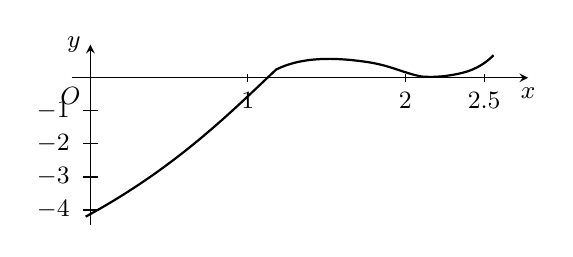
\begin{tikzpicture}[>=stealth,font=\small,x=2.0cm,y=0.42cm]
  \draw[->] (-0.12,0) -- (2.78,0) node[below] {$x$};
  \draw[->] (0,-4.45) -- (0,1.0) node[left] {$y$};
  \node[below left] at (0,0) {$O$};
  \draw[thick] (-0.03,-4.2)
    .. controls (0.55,-2.7) and (0.9,-1.0) .. (1.18,0.25)
    .. controls (1.32,0.58) and (1.5,0.64) .. (1.72,0.5)
    .. controls (1.9,0.4) and (1.98,0.15) .. (2.1,0.04)
    .. controls (2.2,-0.01) and (2.32,0.08) .. (2.4,0.2)
    .. controls (2.48,0.34) and (2.52,0.5) .. (2.56,0.68);
  \foreach \y/\l in {-1/-1,-2/-2,-3/-3,-4/-4}{
    \draw (0.05,\y) -- (-0.05,\y);
    \node[left] at (-0.07,\y) {$\l$};
  }
  \foreach \x/\l in {1/1,2/2,2.5/2.5}{
    \draw (\x,0.12) -- (\x,-0.12);
    \node[below] at (\x,-0.16) {$\l$};
  }
\end{tikzpicture}
\caption{}\label{fig:3.5.2}
\end{figure}

\begin{theorem}\label{thm:3.5.7}
设 $f$ 在区间 $I$ 上连续, 且只有惟一的极值点 $x_{0}$.

(1) 如果 $x_{0}$ 为 $f$ 的极大值点, 则 $x_{0}$ 为 $f$ 的惟一的最大值点;

(2) 如果 $x_{0}$ 为 $f$ 的极小值点, 则 $x_{0}$ 为 $f$ 的惟一的最小值点.
\end{theorem}

\begin{proof}
(1) (反证) 假设有 $x_{1}\neq x_{0}$, $x_{1}\in I$, 使 $f(x_{1})\geqslant f(x_{0})$, 不妨设 $x_{1}>x_{0}$. 由于 $f$ 在 $[x_{0},x_{1}]$ 上连续, 则它必有最小值. 因为 $x_{0}$ 为 $f$ 的极大值, 故 $\exists\delta>0$, 使得
\[
f(x)\leqslant f(x_{0}),\quad\forall x\in[x_{0},x_{0}+\delta),
\]
则必有 $x'\in(x_{0},x_{0}+\delta)$, 使 $f(x')<f(x_{0})$ (否则 $f(x)\equiv f(x_{0})$, $\forall x\in(x_{0},x_{0}+\delta)$, 从而 $(x_{0},x_{0}+\delta)$ 中任何点均为 $f$ 的极值点, 这与只有惟一的极值点 $x_{0}$ 相矛盾). 由以上讨论知, $x_{0}$ 与 $x_{1}$ 均不为 $f$ 在 $[x_{0},x_{1}]$ 中的最小值点. 其最小值点 $\xi\in(x_{0},x_{1})$, 当然 $\xi$ 为 $f$ 的极小值点, 这与 $x_{0}$ 为 $f$ 的惟一的极值点相矛盾.

(2) 可类似(1)证明, 或用 $-f$ 代替 $f$ 即可证得.
\end{proof}

\begin{example}\label{ex:3.5.11}
设 $m>0$, $n>0$, 则当 $0\leqslant x\leqslant a$ 时, 有
\[
x^{m}(a-x)^{n}\leqslant\frac{m^{m}n^{n}}{(m+n)^{m+n}}a^{m+n}.
\]
\end{example}

\begin{proof}
设 $f(x)=x^{m}(a-x)^{n}$, $0\leqslant x\leqslant a$, 则 $f(x)\geqslant 0$, 且
\[
\begin{aligned}
f'(x)&=mx^{m-1}(a-x)^{n}-nx^{m}(a-x)^{n-1}\\
&=x^{m-1}(a-x)^{n-1}[m(a-x)-nx]\\
&=x^{m-1}(a-x)^{n-1}[ma-(m+n)x]
\left\{
\begin{aligned}
&>0,\ 0\leqslant x<\frac{ma}{m+n},\quad f\ \text{单调增},\\
&=0,\ x=\frac{ma}{m+n},\quad f\ \text{取最大值},\\
&<0,\ \frac{ma}{m+n}<x\leqslant a,\quad f\ \text{单调减}.
\end{aligned}
\right.
\end{aligned}
\]
于是,
\[
\begin{aligned}
x^{m}(a-x)^{n}&=f(x)\leqslant f\Big(\frac{ma}{m+n}\Big)\\
&=\Big(\frac{ma}{m+n}\Big)^{m}\Big(a-\frac{ma}{m+n}\Big)^{n}\\
&=\frac{m^{m}}{(m+n)^{m}}\,\frac{n^{n}}{(m+n)^{n}}\,a^{m+n}\\
&=\frac{m^{n}n^{n}}{(m+n)^{m+n}}\,a^{m+n}.
\end{aligned}
\]
\end{proof}

\begin{example}\label{ex:3.5.12}
$1$, $\sqrt{2}=2^{\frac{1}{2}}$, $\sqrt[3]{3}=3^{\frac{1}{3}}$, $\cdots$, $\sqrt[n]{n}=n^{\frac{1}{n}}$, $\cdots$ 中哪一项最大.
\end{example}

\begin{solution}
令 $f(x)=x^{\frac{1}{x}}$, $x>0$, 则
\[
\begin{aligned}
f'(x)&=\big(\mathrm{e}^{\frac{1}{x}\ln x}\big)'=\mathrm{e}^{\frac{1}{x}\ln x}\Big(\frac{-1}{x^{2}}\ln x+\frac{1}{x}\cdot\frac{1}{x}\Big)\\
&=x^{\frac{1}{x}-2}(1-\ln x)
\left\{
\begin{aligned}
&>0,\quad 0<x<\mathrm{e},\ f\ \text{严格增},\\
&=0,\quad x=\mathrm{e},\ f\ \text{达最大值},\\
&<0,\quad x>\mathrm{e},\ f\ \text{严格减}.
\end{aligned}
\right.
\end{aligned}
\]
\[
\lim_{x\to 0^{+}}x^{\frac{1}{x}}=\lim_{x\to 0^{+}}\mathrm{e}^{\frac{1}{x}\ln x}=0,
\]
\[
\lim_{x\to+\infty}x^{\frac{1}{x}}=\mathrm{e}^{\lim\limits_{x\to+\infty}\frac{\ln x}{x}}=\mathrm{e}^{0}=1.
\]
由图~\ref{fig:3.5.3} 知, $\max\limits_{n\in\mathbb{N}}\sqrt[n]{n}=\max\limits_{n\in\mathbb{N}}n^{\frac{1}{n}}=\max\{\sqrt{2},\sqrt[3]{3}\}$, 所以 $\sqrt[3]{3}$ 为最大项.
\end{solution}

\begin{figure}[htbp]
\centering
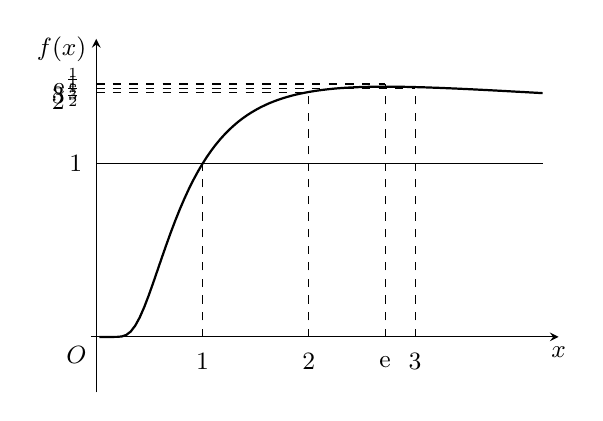
\begin{tikzpicture}[>=stealth,font=\small,x=1.35cm,y=2.2cm]
  \draw[->] (-0.05,0) -- (4.35,0) node[below] {$x$};
  \draw[->] (0,-0.32) -- (0,1.72);
  \node[left] at (0,1.66) {$f(x)$};
  \node[below left] at (0,0) {$O$};
  \draw (0,1) -- (4.2,1);
  \draw[thick] plot[domain=0.03:4.2,samples=100] (\x,{exp(ln(\x)/\x)});
  \draw[dashed] (1,0) -- (1,1);
  \draw[dashed] (2,0) -- (2,1.41);
  \draw[dashed] (2.71828,0) -- (2.71828,1.46);
  \draw[dashed] (3,0) -- (3,1.435);
  \draw[dashed] (0,1.41) -- (2,1.41);
  \draw[dashed] (0,1.46) -- (2.71828,1.46);
  \draw[dashed] (0,1.435) -- (3,1.435);
  \node[left] at (-0.04,1) {$1$};
  \node[left] at (-0.04,1.385) {$2^{\frac{1}{2}}$};
  \node[left] at (-0.04,1.425) {$3^{\frac{1}{3}}$};
  \node[left] at (-0.04,1.475) {$\mathrm{e}^{\frac{1}{\mathrm{e}}}$};
  \foreach \x/\l in {1/1,2/2,3/3}{
    \node[below] at (\x,-0.04) {$\l$};
  }
  \node[below] at (2.71828,-0.06) {$\mathrm{e}$};
\end{tikzpicture}
\caption{}\label{fig:3.5.3}
\end{figure}

\begin{example}\label{ex:3.5.13}
有长方形纸板, 长 8cm, 宽 5cm, 将四角各剪去大小相同的小正方形, 制成无盖纸盒. 问小正方形的边长为多少时, 盒子的容积最大.
\end{example}

\begin{solution}
设剪去的小正方形边长为 $x$, 则 $0<x<\frac{5}{2}$ (如图~\ref{fig:3.5.4} 所示). 纸盒容积为
\[
V=x(8-2x)(5-2x)=4x^{3}-26x^{2}+40x,
\]
\[
V'=12x^{2}-52x+40=4(3x-10)(x-1)
\]
所以, 在 $\left(0,\frac{5}{2}\right)$ 中 $V$ 的驻点为 1. 由
\[
V(0)=0,\ V(1)=18,\ V\Big(\frac{5}{2}\Big)=0
\]
知, 当 $x=1$(cm) 时, 容积 $V(1)=18$(cm$^{3}$) 为最大.
\end{solution}

\begin{figure}[htbp]
\centering
\begin{tikzpicture}[>=stealth,font=\small,scale=0.62]
  \draw[thick] (0,0) rectangle (8,5);
  \fill[pattern=north east lines] (0,0) rectangle (0.85,0.85);
  \fill[pattern=north east lines] (7.15,0) rectangle (8,0.85);
  \fill[pattern=north east lines] (0,4.15) rectangle (0.85,5);
  \fill[pattern=north east lines] (7.15,4.15) rectangle (8,5);
  \draw[decorate,decoration={brace,amplitude=4pt}] (0,5.15) -- (0.85,5.15);
  \node[above] at (0.42,5.2) {$x$};
  \draw[decorate,decoration={brace,amplitude=5pt}] (8.2,0) -- (8.2,5);
  \node[right,rotate=90] at (8.55,2.5) {$5\mathrm{cm}$};
  \draw[decorate,decoration={brace,amplitude=5pt,mirror}] (0,-0.22) -- (8,-0.22);
  \node[below] at (4,-0.34) {$8\mathrm{cm}$};
\end{tikzpicture}
\caption{}\label{fig:3.5.4}
\end{figure}

\begin{example}\label{ex:3.5.14}
设 $A$ 为铁路上一站, 从 $A$ 运原料到工厂 $C$, $C$ 距铁路的垂直距离为 $BC=20$km, $B$ 距 $A$ 的距离 $AB=150$km. 现欲在 $AB$ 之间找一点 $D$, 修公路与 $C$ 连接 (见图~\ref{fig:3.5.5}). 已知铁路运输与公路运输费用之比为 $3:5$. 问: $D$ 修在何处才能使运费最省.
\end{example}

\begin{solution}
设公路运费为 5, 则铁路运费为 3, 置 $D$ 于离 $B$ $x$ (单位: km) 处, 则运费
\[
y=f(x)=3(150-x)+5\sqrt{x^{2}+20^{2}},
\]
\[
0=f'(x)=-3+\frac{5x}{\sqrt{x^{2}+400}},
\]
\[
5x=3\sqrt{x^{2}+400},\ 25x^{2}=9x^{2}+3600,
\]
\[
16x^{2}=3600,\quad x=\pm 15.
\]
因此, 从
\[
f'(x)=-3+\frac{5x}{\sqrt{x^{2}+400}}
\left\{
\begin{aligned}
&<0,\quad x<15,\ f(x)\ \text{严格减},\\
&=0,\quad x=15,\ f(15)\ \text{为最小值},\\
&>0,\quad x>15,\ f(x)\ \text{严格增}
\end{aligned}
\right.
\]
可知 $f(x)$ 在 $x=15$ 达到最小值, 即 $D$ 应选在 $A$ 点与 $B$ 点之间距 $B$ 点 15km 处, 其运费最省 (如图~\ref{fig:3.5.5} 所示). 或者从
\[
f''(x)=\frac{1}{x^{2}+400}\left(\sqrt{x^{2}+400}-\frac{x^{2}}{\sqrt{x^{2}+400}}\right)=\frac{2000}{(x^{2}+400)^{3/2}}>0
\]
得到 $f'(x)$ 严格增, 再由 $f'(15)=0$ 推出
\[
f'(x)\left\{
\begin{aligned}
&<0,\quad x<15,\ f(x)\ \text{严格减},\\
&=0,\quad x=15,\ f(15)\ \text{为最小值},\\
&>0,\quad x>15,\ f(x)\ \text{严格增}.
\end{aligned}
\right.
\]
\end{solution}

\begin{figure}[htbp]
\centering
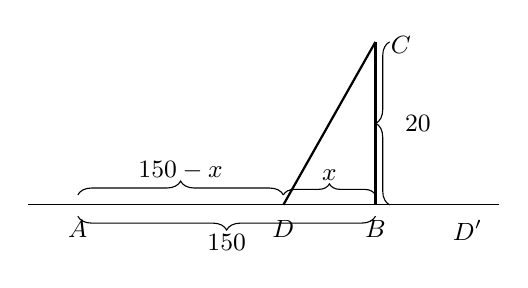
\begin{tikzpicture}[>=stealth,font=\small,scale=0.9]
  \draw (-0.35,0) -- (6.3,0);
  \draw[thick] (4.55,0) -- (4.55,2.3);
  \draw[thick] (3.25,0) -- (4.55,2.3);
  \draw[decorate,decoration={brace,amplitude=5pt}] (0.35,0.14) -- (3.25,0.14);
  \node[above] at (1.8,0.22) {$150-x$};
  \draw[decorate,decoration={brace,amplitude=4pt}] (3.25,0.14) -- (4.55,0.14);
  \node[above] at (3.9,0.2) {$x$};
  \draw[decorate,decoration={brace,amplitude=5pt}] (4.75,0) -- (4.75,2.3);
  \node[right] at (4.83,1.15) {$20$};
  \draw[decorate,decoration={brace,amplitude=5pt,mirror}] (0.35,-0.16) -- (4.55,-0.16);
  \node[below] at (2.45,-0.28) {$150$};
  \node[below] at (0.35,-0.08) {$A$};
  \node[below] at (3.25,-0.08) {$D$};
  \node[below] at (4.55,-0.08) {$B$};
  \node[below] at (5.85,-0.08) {$D'$};
  \node[right] at (4.63,2.25) {$C$};
\end{tikzpicture}
\caption{}\label{fig:3.5.5}
\end{figure}

\begin{example}\label{ex:3.5.15}
证明: 光线的入射角 $\theta_{\text{入}}$ 等于反射角 $\theta_{\text{反}}$.
\end{example}

\begin{proof}
光线服从``最短原理'': 光线从 $(0,a)$ 经 $x$ 轴上某点 $(x,0)$ 反射到 $(b,c)$ 点 (如图~\ref{fig:3.5.6} 所示). $x$ 在何处时, 所走路程 $AB+BC$ 最短.

设
\[
L(x)=AB+BC=\sqrt{a^{2}+x^{2}}+\sqrt{(b-x)^{2}+c^{2}}
\]
则
\[
L'(x)=\frac{x}{\sqrt{a^{2}+x^{2}}}-\frac{b-x}{\sqrt{(b-x)^{2}+c^{2}}},\quad 0\leqslant x\leqslant b,
\]
\[
\begin{aligned}
L''(x)&=\frac{1}{\sqrt{a^{2}+x^{2}}}-\frac{x^{2}}{\sqrt{(a^{2}+x^{2})^{3/2}}}+\frac{1}{\sqrt{(b-x)^{2}+c^{2}}}\\
&\quad-\frac{(b-x)^{2}}{\left[(b-x)^{2}+c^{2}\right]^{3/2}}\\
&=\frac{a^{2}+x^{2}-x^{2}}{(a^{2}+x^{2})^{3/2}}+\frac{(b-x)^{2}+c^{2}-(b-x)^{2}}{\left[(b-x)^{2}+c^{2}\right]^{3/2}}\\
&=\frac{a^{2}}{(a^{2}+x^{2})^{3/2}}+\frac{c^{2}}{\left[(b-x)^{2}+c^{2}\right]^{3/2}}>0.
\end{aligned}
\]
从而 $L'(x)$ 严格增, 且 $L(x)$ 在驻点 $\left(\frac{x}{\sqrt{a^{2}+x^{2}}}=\frac{b-x}{\sqrt{(b-x)^{2}+c^{2}}}\Longleftrightarrow\frac{a^{2}}{x^{2}}=\frac{c^{2}}{(b-x)^{2}}\Longleftrightarrow x=\frac{ab}{a+c}\right)$ 处达到最小值. 此时, $\triangle AOB\sim\triangle CDB$, 即 $\theta_{\text{入}}=\theta_{\text{反}}$.
\end{proof}

\begin{figure}[htbp]
\centering
\begin{tikzpicture}[>=stealth,font=\small,scale=1.0]
  \draw[->] (-0.1,0) -- (3.4,0) node[below] {$x$};
  \draw[->] (0,-0.12) -- (0,2.75);
  \node[left] at (0,2.68) {$y$};
  \node[below left] at (0,0) {$O$};
  \draw (2.95,0) -- (2.95,2.35);
  \draw[->] (0,2.0) -- (1.05,0);
  \draw[->] (1.05,0) -- (2.95,2.35);
  \draw[dashed] (1.05,0) -- (1.05,2.2);
  \draw (1.05,0.5) arc[start angle=90,end angle=117.7,radius=0.5];
  \draw (1.05,0.62) arc[start angle=50.3,end angle=90,radius=0.62];
  \node at (0.66,0.66) {$\theta_{\text{入}}$};
  \node at (1.5,0.86) {$\theta_{\text{反}}$};
  \node[above right] at (0,1.95) {$A(0,a)$};
  \node[below] at (1.05,-0.1) {$B(x,0)$};
  \node[below] at (2.95,-0.1) {$D(b,0)$};
  \node[right] at (2.99,2.35) {$C(b,c)$};
\end{tikzpicture}
\caption{}\label{fig:3.5.6}
\end{figure}

\begin{example}\label{ex:3.5.16}
炼油厂要修建容量为 $V_{0}$ 的贮油罐. 问: 此罐的底面直径与高之比为多少时, 用料量最省即表面积最小.
\end{example}

\begin{solution}
设油罐底面半径为 $r$, 高为 $h$, 则
\[
S=2\pi rh+2\pi r^{2}
\]
\[
V_{0}=\pi r^{2}h,\quad h=\frac{V_{0}}{\pi r^{2}},\quad r>0.
\]
于是,
\[
S=2\pi r\cdot\frac{V_{0}}{\pi r^{2}}+2\pi r^{2}=\frac{2V_{0}}{r}+2\pi r^{2},\quad r>0.
\]
\[
\begin{aligned}
S'&=-\frac{2V_{0}}{r^{2}}+4\pi r\\
&=\frac{2}{r^{2}}(2\pi r^{3}-V_{0})
\left\{
\begin{aligned}
&<0,\quad 0<r<\sqrt[3]{\frac{V_{0}}{2\pi}},\ S(r)\ \text{严格减},\\
&=0,\quad r=\sqrt[3]{\frac{V_{0}}{2\pi}},\ S\Big(\sqrt[3]{\frac{V_{0}}{2\pi}}\Big)\ \text{为最小值},\\
&>0,\quad r>\sqrt[3]{\frac{V_{0}}{2\pi}},\ S(r)\ \text{严格增},
\end{aligned}
\right.
\end{aligned}
\]
即当 $\frac{2r}{h}=\frac{2r}{\frac{V_{0}}{\pi r^{2}}}=\frac{2\pi r^{3}}{V_{0}}=\frac{2\pi\cdot\frac{V_{0}}{2\pi}}{V_{0}}=1$ 时, 表面积最省.
\end{solution}

\begin{exblock}{练习题 3.5}
  \item 确定下列函数的单调区间:
  \begin{enumerate}[label=(\arabic*)]
    \item $f(x)=3x-x^{2}$;
    \item $f(x)=2x^{2}-\ln x$;
    \item $f(x)=\sqrt{2x-x^{2}}$;
    \item $f(x)=\frac{x^{2}-1}{x}$;
    \item $f(x)=\arctan x-x$.
  \end{enumerate}

  \item 应用函数的单调性证明下列不等式:
  \begin{enumerate}[label=(\arabic*)]
    \item $\tan x>x-\frac{x^{3}}{3}$, $x\in\left(0,\frac{\pi}{3}\right)$;
    \item $\frac{2x}{\pi}<\sin x<x$, $x\in\left(0,\frac{\pi}{2}\right)$;
    \item $x-\frac{x^{2}}{2}<\ln(1+x)<x-\frac{x^{2}}{2(1+x)}$;
    \item $x(x-\arctan x)>0$, $x\neq 0$;
    \item $\ln(1+x)>\frac{\arctan x}{1+x}$, $x>0$.
  \end{enumerate}

  \item 设 $a,b>0$. 证明: 方程 $x^{3}+ax+b=0$ 不存在正根.

  \item 证明: $\frac{\tan x}{x}>\frac{x}{\sin x}$, $x\in\left(0,\frac{\pi}{2}\right)$.

  \item 设函数 $f$ 与 $g$ 在区间 $[a,+\infty)$ 上连续可导, 且当 $x>a$ 时, $|f'(x)|\leqslant g'(x)$. 证明: 当 $x\geqslant a$ 时,
  \[
  |f(x)-f(a)|\leqslant g(x)-g(a).
\]

  \item 设函数 $y=f(x)$ 在点 $x$ 处 3 阶可导, 且 $f'(x)\neq 0$. 证明: $f(x)$ 严格增或严格减, 从而存在反函数 $x=f^{-1}(y)$. 试用 $f'(x)$, $f''(x)$ 及 $f'''(x)$ 表示 $(f^{-1})''(y)$.

  \item 证明:
  (1) 方程 $x^{3}-3x+c=0$ ($c$ 为常数) 在区间 $[0,1]$ 内不可能有两个不同的实根.

  (2) 方程 $x^{n}+px+q=0$ ($n\in\mathbb{N}$, $p,q\in\mathbb{R}$) 当 $n$ 为偶数时至多有 2 个实根; 当 $n$ 为奇数时至多有 3 个实根.

  \item 设函数 $f$ 在 $[a,b]$ 上可导. 证明:
  (1) 若 $f'(x)\geqslant m$, 则 $f(x)\geqslant f(a)+m(x-a)$, $\forall x\in[a,b]$;

  (2) 若 $|f'(x)|\leqslant M$, 则 $|f(x)-f(a)|\leqslant M(x-a)$, $\forall x\in[a,b]$.

  \item 求下列函数的极值:
  \begin{enumerate}[label=(\arabic*)]
    \item $f(x)=2x^{3}-x^{4}$;
    \item $f(x)=\frac{2x}{1+x^{2}}$;
    \item $f(x)=\frac{(\ln x)^{2}}{x}$;
    \item $f(x)=\arctan x-\frac{1}{2}\ln(1+x^{2})$;
    \item $f(x)=|x(x^{2}-1)|$;
    \item $f(x)=(x-1)^{2}(x+1)^{3}$;
    \item $f(x)=\frac{x(x^{2}+1)}{x^{4}-x^{2}+1}$.
  \end{enumerate}

  \item 设
  \[
  f(x)=\left\{
  \begin{aligned}
  &x^{4}\sin^{2}\frac{1}{x},\quad x\neq 0,\\
  &0,\quad x=0.
  \end{aligned}
  \right.
\]
  (1) 证明: $x=0$ 为 $f$ 的极小值点, 也是最小值点;

  (2) 说明 $f$ 的极小值点 $x=0$ 处是否满足极值的充分条件一或充分条件二.

  \item 求下列函数在给定区间上的最大与最小值:
  \begin{enumerate}[label=(\arabic*)]
    \item $f(x)=x^{4}-2x^{2}+5$, $|x|\leqslant 2$;
    \item $f(x)=x^{5}-5x^{4}+5x^{3}+1$, $x\in[-1,2]$;
    \item $f(x)=x\ln x$, $x>0$;
    \item $f(x)=\sqrt{x}\ln x$, $x>0$;
    \item $f(x)=x^{2}-3x+2$, $x\in\mathbb{R}$;
    \item $f(x)=|x^{2}-3x+2|$, $|x|\leqslant 10$;
    \item $f(x)=2\tan x-\tan^{2}x$, $x\in\left[0,\frac{\pi}{2}\right)$;
    \item $f(x)=\arctan\frac{1-x}{1+x}$, $0\leqslant x\leqslant 1$.
  \end{enumerate}

  \item 设函数 $f$ 在点 $x_{0}$ 处有 $f'_{+}(x_{0})<0\,(>0)$, $f'_{-}(x_{0})>0\,(<0)$, 则 $x_{0}$ 为 $f$ 极大(小)值点.

  \item 证明: 当 $x>0$ 且 $x\neq 1$ 时, 有 $(1-x)\big(x^{2}\mathrm{e}^{\frac{1}{x}}-\mathrm{e}^{x}\big)>0$ (提示: 考察 $\varphi(x)=2\ln x+\frac{1}{x}-x$).

  \item 求一正数 $x$, 使它与其倒数之和 $f(x)=x+\frac{1}{x}$ 最小.

  \item 证明: (1) 周长为 $l$ 的矩形中, 以正方形所围面积最大; (2) 面积为定值 $S$ 的矩形中, 以正方形的边长为最小.

  \item 设用某仪器进行测量时, 读得 $n$ 次实验数据为 $a_{1},a_{2},\cdots,a_{n}$. 问以怎样的数值 $x$ 表达所要测量的真值, 才能使它与这 $n$ 个数之差的平方和为最小 (提示: 即证 $f(x)=\sum\limits_{i=1}^{n}(x-a_{i})^{2}$ 的最小值为 $\bar{x}=\frac{a_{1}+a_{2}+\cdots+a_{n}}{n}$).

  \item 内接于椭圆 $\frac{x^{2}}{a^{2}}+\frac{y^{2}}{b^{2}}=1$, 边平行于坐标轴的矩形, 何时面积最大.

  \item 从半径为 $R$ 的圆纸片上剪去一个扇形, 做成一个圆锥形的漏斗. 如何选取扇形的顶角, 可使漏斗的容积最大.

  \item 设 $0<a<b\leqslant 2a$, 在区间 $[a,b]$ 上讨论双曲线 $xy=1$. 在该曲线每一点上作切线, 它与横轴及两平行直线 $x=a$, $x=b$ 围成一个梯形. 问这切线位于何处, 才能使梯形有最大面积.

  \item 在抛物线 $y^{2}=2px$ 上哪一点的法线被抛物线所截之线段为最短.

  \item 有一个无盖的圆柱形容器, 当给定体积为 $V_{0}$ 时, 要使容器的表面积为最小, 问底的半径与容器高的比例为多大.

  \item 要将货物从运河边上 $A$ 城运往与运河相距 $a$ (单位: km) 的 $B$ 城, 轮船运费的单价是 $\alpha$ 元/km, 火车运费的单价是 $\beta$ 元/km ($\beta>\alpha$). 试求运河边上的一点 $M$, 修建铁路 $MB$, 使总运费最省.

  \item 重量为 $W$ 的物体放在一粗糙的平面上, 施加一力克服摩擦, 使之在平面上滑动, 其摩擦系数为 $\mu$, 问该力应与水平成何角度, 方可使用力最小?

  \item 设 $f(x)=a\ln x+bx^{2}+x$ 在 $x_{1}=1$, $x_{2}=2$ 处都取得极值, 试求 $a$ 与 $b$; 并问此时 $f$ 在 $x_{1}$ 与 $x_{2}$ 是取得极大值还是极小值.

  \item 证明: 定圆内接正 $n$ 边形面积随 $n$ 的增加而增加.

  \item 讨论函数
  \[
  f(x)=\left\{
  \begin{aligned}
  &\frac{x}{2}+x^{2}\sin\frac{1}{x},\quad x\neq 0,\\
  &0,\quad x=0.
  \end{aligned}
  \right.
\]
  (1) 在 $x=0$ 点是否可导.

  (2) 是否存在 $x=0$ 的一个开邻域, 使 $f$ 在该开邻域内单调.

  \item 设 $k>0$. 试问: $k$ 为何值时, 方程 $\arctan x-kx=0$ 有正实根.
\end{exblock}

\begin{exblock}{思考题 3.5}
  \item 设 $0<b<a$. 证明:
  \[
  \frac{a-b}{\sqrt{1+a^{2}}\sqrt{1+b^{2}}}<\arctan a-\arctan b<a-b,\quad\text{其中 } 0<b<a.
\]

  \item 证明下列不等式:
  (1) 当 $0<x_{1}<x_{2}<\frac{\pi}{2}$ 时, 有
  \[
  \frac{\tan x_{2}}{\tan x_{1}}>\frac{x_{2}}{x_{1}};
\]

  (2) 当 $x,y>0$ 且 $\beta>\alpha>0$ 时, 有
  \[
  (x^{\alpha}+y^{\alpha})^{\frac{1}{\alpha}}>(x^{\beta}+y^{\beta})^{\frac{1}{\beta}};
\]

  (3) 设 $p\geqslant 2$, 当 $x\in[0,1]$ 时, 有
  \[
  \left(\frac{1+x}{2}\right)^{p}+\left(\frac{1-x}{2}\right)^{p}\leqslant\frac{1}{2}(1+x^{p}).
\]

  \item 设函数 $f$ 在区间 $[0,+\infty)$ 上可导, $f(0)=0$ 且 $f'$ 严格增. 证明: $\frac{f(x)}{x}$ 在 $(0,+\infty)$ 上也严格增.

  \item 设求出使得不等式 $a^{x}\geqslant x^{a}$ ($x>0$) 成立的一切正数 $a$ (提示: 考察函数 $f(x)=\frac{\ln x}{x}$).

  \item 设 $f$ 在 $[a,+\infty)$ 上 2 阶可导, 且 $f(a)>0$, $f'(a)<0$, 当 $x>a$ 时, $f''(x)\leqslant 0$. 证明: 方程 $f(x)=0$ 在 $(a,+\infty)$ 内有且仅有一根.
\end{exblock}
